\documentclass[a4paper, 12pt]{article}
\usepackage[utf8]{inputenc}
\usepackage[french]{babel}
\usepackage[T1]{fontenc}
\usepackage[top=2cm,bottom=2cm,left=2cm,right=2cm]{geometry}
\usepackage{hyperref}
\usepackage{graphicx}
\usepackage{caption}
\usepackage{sectsty}
\usepackage{xcolor}

\captionsetup{position=below}
\hypersetup{pdfborder = 0 0 0}

% définition des couleurs

\definecolor{color_section}{RGB}{87,68,95}
\definecolor{color_subsection}{RGB}{46,81,159}
\definecolor{color_sub-subsection}{RGB}{121,142,200}

% associer les couleurs aux titres de section

\sectionfont{\color{color_section}\underline}
\subsectionfont{\color{color_subsection}\underline}
\subsubsectionfont{\color{color_sub-subsection}\underline}

% entête

\title{- Rapport de projet - \\ Conception d'un solveur de ricochet robots}

\author{
    \textsc{André} Lorada \\ 
    \textsc{Auvray} Théo \\ 
    \textsc{Auvray} Valentin \\ 
    \textsc{Kachri} Oussama \\ 
Licence 2 informatique - Groupe 1A
}

\date \today

\begin{document}

% logo unicaen

\begin{figure}[t]
    
\includegraphics[scale=1]{images/logo.png}
\end{figure}

\maketitle

% image de départ 

\begin{figure}[ht]
            \centering
            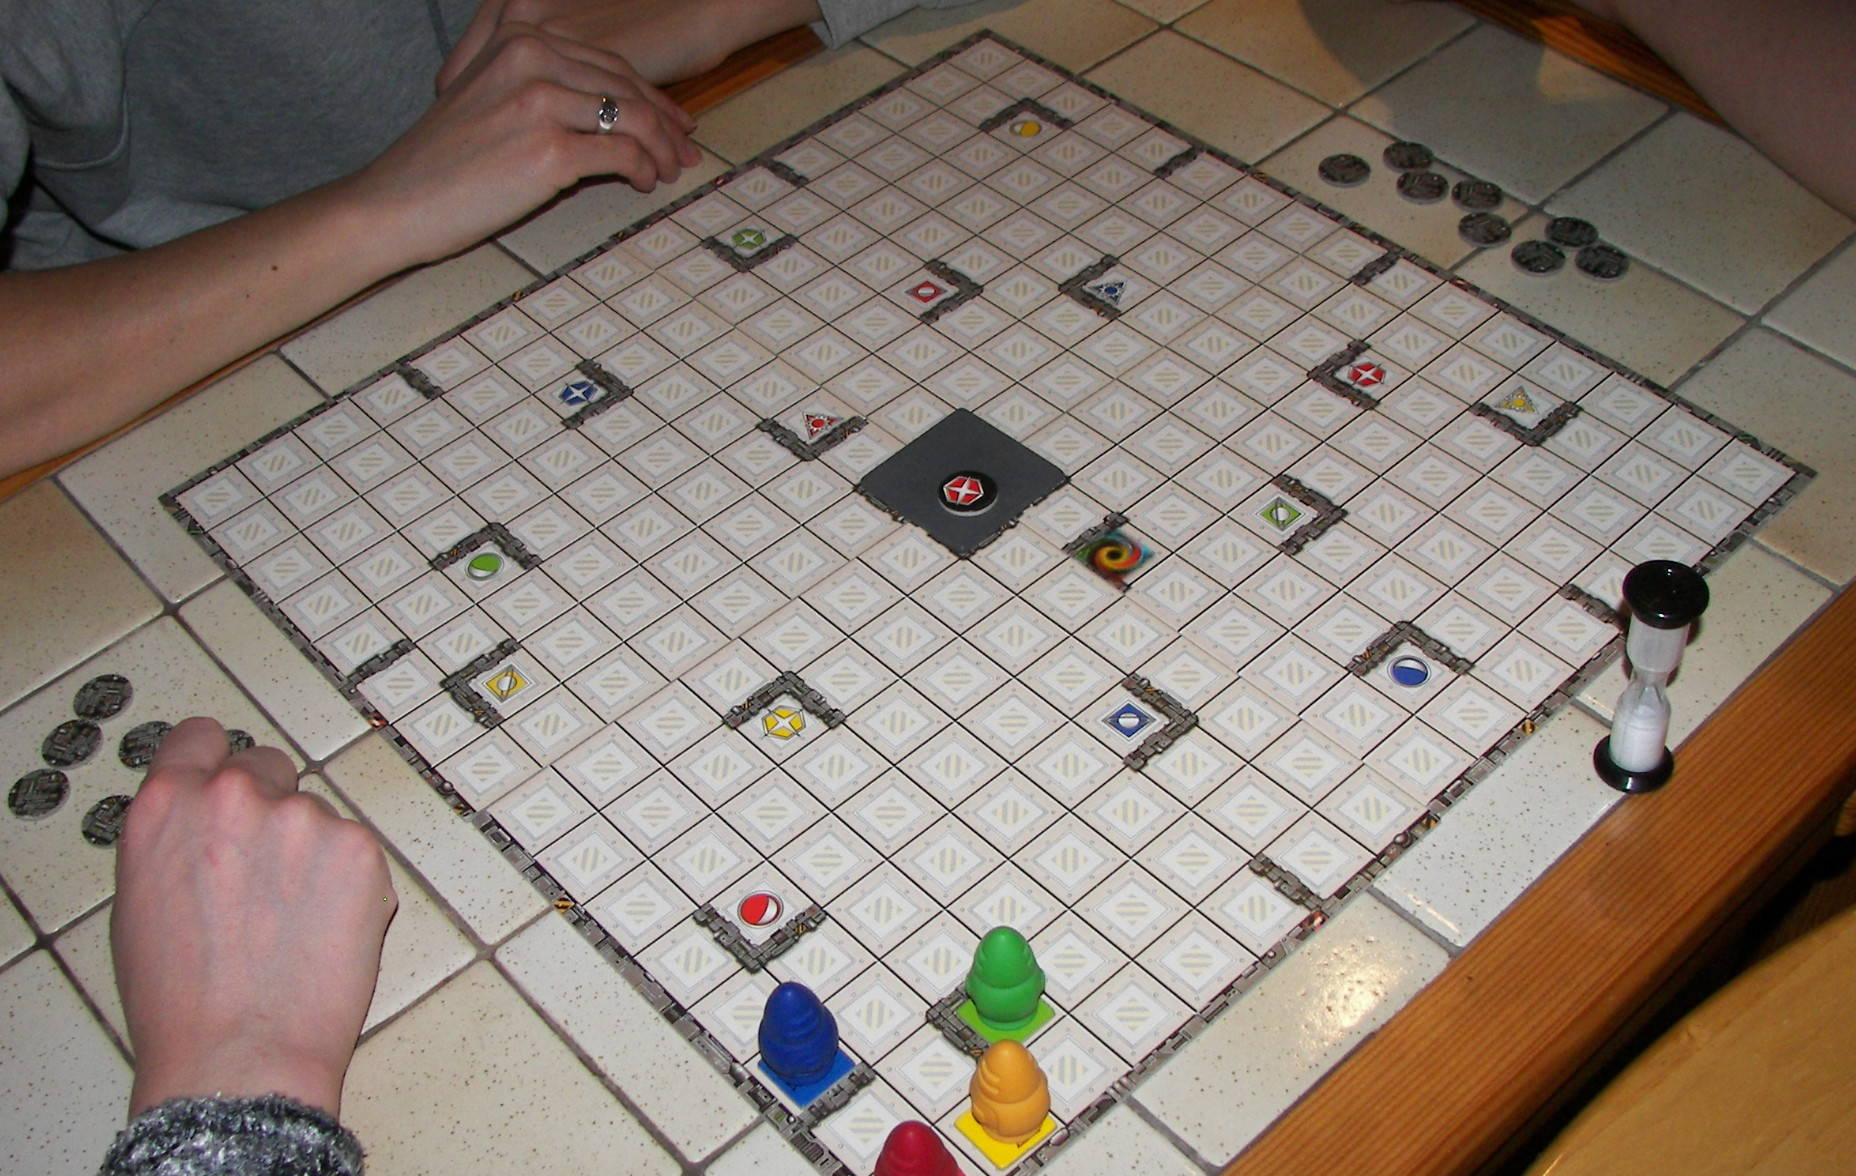
\includegraphics[scale=0.5]{images/ricochetrobot.jpg}
\end{figure}

\newpage

\tableofcontents

\newpage

\section{Introduction}
\section{Organisation du projet}
    \subsection{Gestion du projet}
    \subsection{Répartition des tâches}
\section{Architecture du projet}
    \subsection{Arborescence du projet}
    \subsection{diagramme des modules et des classes}
\section{Éléments techniques}
    \subsection{Description des fonctionnalités}
    \subsection{Implémentation}
    \subsection{Algorithme spécifique}
\section{Pistes et réflexions de certains aspects}
\section{Expérimentation et usage}
\section{Conclusion}
\section{Pistes d'améliorations}
\bibliography{Réferences}
\end{document}
